%%%%%%%%%%%%%%%%%%%%%%%%%%%%%%%%%%%%%%%%%%%%%%%%%%%%%%%%%%%%%%%%%%%%%%%%%%%%%%%%
% TUM-Vorlage: Präsentation
%%%%%%%%%%%%%%%%%%%%%%%%%%%%%%%%%%%%%%%%%%%%%%%%%%%%%%%%%%%%%%%%%%%%%%%%%%%%%%%%
%
% Rechteinhaber:
%     Technische Universität München
%     https://www.tum.de
% 
% Gestaltung:
%     ediundsepp Gestaltungsgesellschaft, München
%     http://www.ediundsepp.de
% 
% Technische Umsetzung:
%     eWorks GmbH, Frankfurt am Main
%     http://www.eworks.de
%
%%%%%%%%%%%%%%%%%%%%%%%%%%%%%%%%%%%%%%%%%%%%%%%%%%%%%%%%%%%%%%%%%%%%%%%%%%%%%%%%


%%%%%%%%%%%%%%%%%%%%%%%%%%%%%%%%%%%%%%%%%%%%%%%%%%%%%%%%%%%%%%%%%%%%%%%%%%%%%%%%
% Zur Wahl des Seitenverhältnisses bitte einen der beiden folgenden Befehle
% auskommentieren und den ausführen lassen:
\documentclass[t]{beamer}
\usepackage[
    orientation=landscape,
    size=custom,
    width=25.4,
    height=19.05,
    scale=0.63 % erzeugt 16pt Schriftgröße
]{beamerposter}

\newcommand{\PraesentationSchriftgroesseSehrGross}{\fontsize{30}{45}}
\newcommand{\PraesentationSchriftgroesseGross}{\fontsize{22}{33}}
\newcommand{\PraesentationSchriftgroesseNormal}{\fontsize{16}{29}}
\newcommand{\PraesentationSchriftgroesseKlein}{\fontsize{12}{18}}
\newcommand{\PraesentationSchriftgroesseDreizeiler}{\fontsize{7}{10}}
\newcommand{\PraesentationSchriftgroesseAufzaehlungszeichen}{\fontsize{10}{8}}

\newcommand{\PraesentationAbstandAbsatz}{22.1pt}
\newcommand{\PraesentationPositionKorrekturOben}{0cm}
\newcommand{\PraesentationBeispieleSchriftgroessen}{30 | 22 | 16 | 12}
\usepackage[utf8]{inputenc}
\usepackage[T1]{fontenc} % Zeichensatzkodierung

\usepackage{calc} % Berechnungen

\usepackage[nenglish]{babel} % Deutsche Lokalisierung
\usepackage{graphicx} % Grafiken
\usepackage[export]{adjustbox}
\usepackage[absolute, overlay]{textpos} % Positionierung

% Silbentrennung:
\usepackage{hyphenat}
%\tolerance 2414
%\hbadness 2414
%\emergencystretch 1.5em
%\hfuzz 0.3pt
%\widowpenalty=10000     % Hurenkinder
%\clubpenalty=10000      % Schusterjungen
%\vfuzz \hfuzz

% Euro-Symbol:
\usepackage[gen]{eurosym}
\DeclareUnicodeCharacter{20AC}{\euro{}}

% Schriftart Helvetica:
\usepackage[scaled]{helvet}
\renewcommand{\familydefault}{\sfdefault}

%\usepackage{mathptmx} % skalierbare Formelschriften

\usepackage{tabularx}

\usepackage{multicol} % mehrspaltiger Text

\usepackage{tikz}
\usetikzlibrary{arrows, shapes, shapes.multipart, trees, positioning,
    backgrounds, fit, matrix}

% Diagramme:
\usepackage{pgfplots}
\pgfplotsset{compat=default}

% Erweiterbare Fusszeile:
\newcommand{\PraesentationFusszeileZusatz}{}
 % Seitenverhältnis 4:3
% \input{./Ressourcen/Praesentation/Praeambel16zu9.tex} % Seitenverhältnis 16:9
%%%%%%%%%%%%%%%%%%%%%%%%%%%%%%%%%%%%%%%%%%%%%%%%%%%%%%%%%%%%%%%%%%%%%%%%%%%%%%%%


%%%%%%%%%%%%%%%%%%%%%%%%%%%%%%%%%%%%%%%%%%%%%%%%%%%%%%%%%%%%%%%%%%%%%%%%%%%%%%%%
%%%%%%%%%%%%%%%%%%%%%%%%%%%%%%%%%%%%%%%%%%%%%%%%%%%%%%%%%%%%%%%%%%%%%%%%%%%%%%%%
% TUM-Vorlage: Personenspezifische Informationen
%%%%%%%%%%%%%%%%%%%%%%%%%%%%%%%%%%%%%%%%%%%%%%%%%%%%%%%%%%%%%%%%%%%%%%%%%%%%%%%%
%
% Rechteinhaber:
%     Technische Universität München
%     https://www.tum.de
% 
% Gestaltung:
%     ediundsepp Gestaltungsgesellschaft, München
%     http://www.ediundsepp.de
% 
% Technische Umsetzung:
%     eWorks GmbH, Frankfurt am Main
%     http://www.eworks.de
%
%%%%%%%%%%%%%%%%%%%%%%%%%%%%%%%%%%%%%%%%%%%%%%%%%%%%%%%%%%%%%%%%%%%%%%%%%%%%%%%%

% Für die Person anpassen:

\newcommand{\PersonVorname}{Raffael}
\newcommand{\PersonNachname}{D\"ull}
\newcommand{\PersonStadt}{Munich}
\newcommand{\PersonAdresse}{}
\newcommand{\PersonTelefon}{}
\newcommand{\PersonFax}{}
\newcommand{\PersonEmail}{raffael.duell@tum.de}
\newcommand{\PersonWebseite}{}

\newcommand{\FakultaetAnsprechpartner}{}
% Fakultät:
\newcommand{\FakultaetName}{Faculty for Informatics}
\newcommand{\LehrstuhlName}{}

\newcommand{\EinstellungBankName}{}
\newcommand{\EinstellungBankIBAN}{}
\newcommand{\EinstellungBankBIC}{}
\newcommand{\EinstellungSteuernummer}{}
\newcommand{\EinstellungUmsatzsteuerIdentifikationsnummer}{}

\hyphenation{} % eigene Silbentrennung                    % !!! DATEI ANPASSEN !!!
%%%%%%%%%%%%%%%%%%%%%%%%%%%%%%%%%%%%%%%%%%%%%%%%%%%%%%%%%%%%%%%%%%%%%%%%%%%%%%%%

\usepackage{amsmath}
\usepackage{bm}
\definecolor{princetonorange}{rgb}{1.0, 0.56, 0.0}
\newcommand{\Datum}{\today}

\renewcommand{\PraesentationFusszeileZusatz}{| Seminar WaveSim | Topic 8: Source terms}

\title{Topic 8: Source terms}
\author{\PersonTitel{} \PersonVorname{} \PersonNachname}
\institute[]{\UniversitaetName \\ \FakultaetName \\ \LehrstuhlName}
\date[\Datum]{Munich, 30 January 2020}
\subject{Thema der Präsentation}


%%%%%%%%%%%%%%%%%%%%%%%%%%%%%%%%%%%%%%%%%%%%%%%%%%%%%%%%%%%%%%%%%%%%%%%%%%%%%%%%
%%%%%%%%%%%%%%%%%%%%%%%%%%%%%%%%%%%%%%%%%%%%%%%%%%%%%%%%%%%%%%%%%%%%%%%%%%%%%%%%
% EINSTELLUNGEN
%%%%%%%%%%%%%%%%%%%%%%%%%%%%%%%%%%%%%%%%%%%%%%%%%%%%%%%%%%%%%%%%%%%%%%%%%%%%%%%%

% Allgemein:
\newcommand{\AllgemeinGestalter}{ediundsepp Gestaltungsgesellschaft}
\newcommand{\AllgemeinErsteller}{eWorks GmbH}

% Universität:
\newcommand{\UniversitaetName}{Technische Universität München}
\newcommand{\UniversitaetAbkuerzung}{TUM}
\newcommand{\UniversitaetWebseite}{www.tum.de}
\newcommand{\UniversitaetLogoBreite}{19mm}
\newcommand{\UniversitaetLogoHoehe}{1cm}

\newcommand{\UniversitaetAdresse}{%
    Arcisstraße~21\\%
    80333~München%
}

\newcommand{\PraesentationSeitenrand}{8.9mm}
\newcommand\crule[3][black]{\textcolor{#1}{\rule{#2}{#3}}}

\newlength\smallerbaselineskip
\setlength{\smallerbaselineskip}{0.8\baselineskip}

    % Blautöne:
\definecolor{TUMBlau}{RGB}{0,101,189} % Pantone 300
\definecolor{TUMBlauDunkel}{RGB}{0,82,147} % Pantone 301
\definecolor{TUMBlauHell}{RGB}{152,198,234} % Pantone 283
\definecolor{TUMBlauMittel}{RGB}{100,160,200} % Pantone 542

    % Hervorhebung:
\definecolor{TUMElfenbein}{RGB}{218,215,203} % Pantone 7527 -Elfenbein
\definecolor{TUMGruen}{RGB}{162,173,0} % Pantone 383 - Grün
\definecolor{TUMOrange}{RGB}{227,114,34} % Pantone 158 - Orange
\definecolor{TUMGrau}{gray}{0.6} % Grau 60%


\setbeamercolor*{alerted text}{fg=TUMOrange}

\newcommand{\PraesentationSetzeTextfarbe}{%
    \color{PraesentationTextfarbe}%
    \setbeamercolor*{frametitle}{fg=PraesentationTextfarbe}%
    \setbeamercolor*{normal text}{fg=PraesentationTextfarbe}%
    \setbeamercolor{itemize/enumerate body}{fg=PraesentationTextfarbe}%
    \setbeamercolor*{itemize item}{fg=PraesentationTextfarbe}%
}

\newcommand{\PraesentationFarbschemaStandard}{%
    \setbeamercolor*{background canvas}{}%
    \definecolor{PraesentationTextfarbe}{rgb}{0,0,0}%
    \PraesentationSetzeTextfarbe%
}

\newcommand{\PraesentationFarbschemaWeissBlau}{%
    \setbeamercolor*{background canvas}{bg=TUMBlauDunkel}%
    \definecolor{PraesentationTextfarbe}{rgb}{1,1,1}%
    \PraesentationSetzeTextfarbe%
}

\newcommand{\PraesentationFarbschemaWeissSchwarz}{%
    \setbeamercolor*{background canvas}{bg=black}%
    \definecolor{PraesentationTextfarbe}{rgb}{1,1,1}%
    \PraesentationSetzeTextfarbe%
}

\newcommand{\PraesentationTitelseiteInhalt}{%
    \begin{textblock*}{\paperwidth}[0,0](0cm,-\PraesentationSeitenrand - 6.5mm + \PraesentationPositionKorrekturOben)%
        \color{PraesentationTextfarbe}%
        \frametitle{\inserttitle}
        \vspace*{49.4mm}%
        \usebeamerfont{author}\selectfont\insertauthor\\%
        \insertinstitute\\%
        \insertdate%
    \end{textblock*}%
}

\newcommand{\PraesentationSeitenkopfInhalt}[1]{%
    %\vspace*{31.7mm}%
    \begin{textblock*}{1.68cm}[1,0](\paperwidth - \PraesentationSeitenrand - \PraesentationSeitenrand, 0cm)%
        \includegraphics[width=1.68cm]{#1}%
    \end{textblock*}%
    \begin{textblock*}{3cm}[1,0](\paperwidth - \PraesentationSeitenrand, -\PraesentationSeitenrand)%
        \hbox{%
            \color{PraesentationTextfarbe}%
            \hbox{\insertframenavigationsymbol}%
            \hbox{\insertsubsectionnavigationsymbol}%
            \hbox{\insertsectionnavigationsymbol}%
        }%
    \end{textblock*}%
}

\newcommand{\PraesentationBildUhrenturm}{%
    \begin{textblock*}{10.82cm}[1,1](\paperwidth - \PraesentationSeitenrand - \PraesentationSeitenrand, \paperheight - 9mm)%
        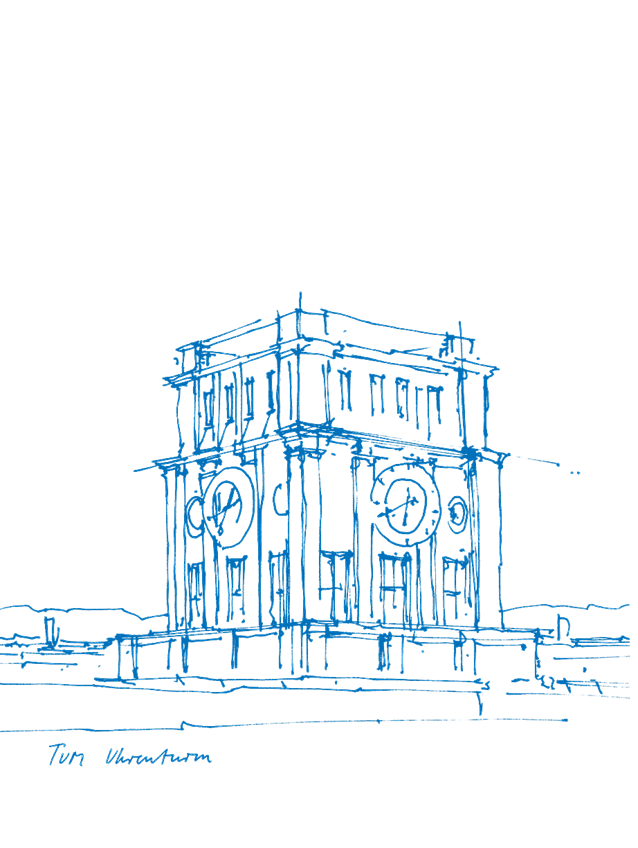
\includegraphics{figures/TUM_Uhrenturm.png}%
    \end{textblock*}%
}

\newcommand{\PraesentationStartseiteUhrenturm}{%
    \setbeamertemplate{title page}{%
        \PraesentationSeitenkopfInhalt{figures/Universitaet_Logo_RGB.pdf}%
        \PraesentationBildUhrenturm%
        \PraesentationTitelseiteInhalt%
    }%
}

\newcommand{\PraesentationStartseiteFlaggen}{%
    \setbeamertemplate{title page}{%
        \begin{textblock*}{\paperwidth}[0,1](-\PraesentationSeitenrand,\paperheight-\PraesentationSeitenrand)%
            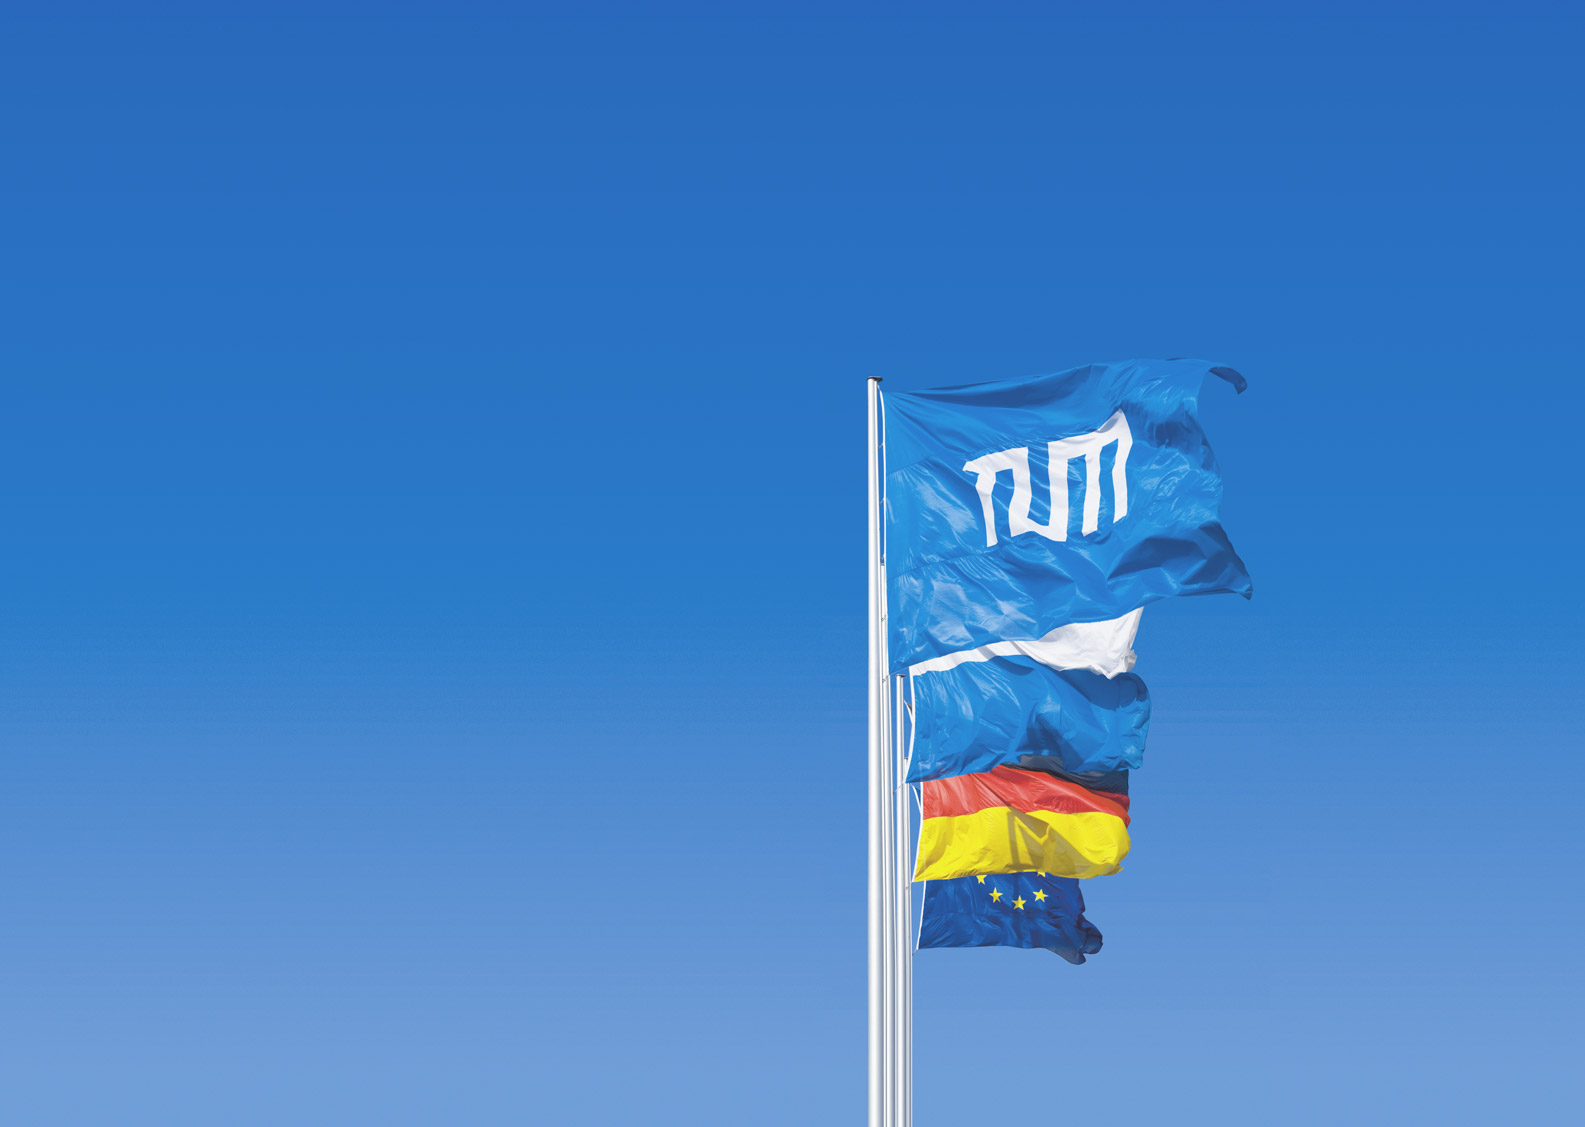
\includegraphics[min width=\paperwidth,max width=\paperheight,min totalsize={\paperwidth}{\paperheight},keepaspectratio,center]{figures/Universitaet_Flaggen.jpg}%
        \end{textblock*}%
        \PraesentationSeitenkopfInhalt{figures/Universitaet_Logo_weiss.pdf}%
        \PraesentationTitelseiteInhalt%
    }%
}

\newcommand{\PraesentationStartseiteLeer}{%
    \setbeamertemplate{title page}{%
        \PraesentationSeitenkopfInhalt{figures/Universitaet_Logo_weiss.pdf}%
        \PraesentationTitelseiteInhalt%
    }%
}


\newcommand{\PraesentationMasterStandard}{%
    \PraesentationFarbschemaStandard%
    \PraesentationStartseiteUhrenturm%
    \setbeamertemplate{headline}{%
        \PraesentationSeitenkopfInhalt{figures/Universitaet_Logo_RGB.pdf}%
    }%
}

\newcommand{\PraesentationMasterWeissBlau}{%
    \PraesentationFarbschemaWeissBlau%
    \PraesentationStartseiteLeer%
    \setbeamertemplate{headline}{%
        \PraesentationSeitenkopfInhalt{figures/Universitaet_Logo_weiss.pdf}%
    }%
}


\newcommand{\PraesentationMasterKopfzeileDreizeiler}{%
    \PraesentationFarbschemaStandard%
    \setbeamertemplate{title page}{%
        \begin{textblock*}{\paperwidth}[0,0](0cm, -7.8mm)%
            \color{TUMBlau}\PraesentationSchriftgroesseDreizeiler\selectfont%
            \LehrstuhlName\\%
            \FakultaetName\\%
            \UniversitaetName\vskip0pt%
            \normalcolor\normalsize\selectfont%
        \end{textblock*}%
        \PraesentationSeitenkopfInhalt{figures/Universitaet_Logo_RGB.pdf}%
        \PraesentationBildUhrenturm%
        \PraesentationTitelseiteInhalt%
    }%
    \setbeamertemplate{headline}{%
        \begin{textblock*}{\paperwidth}[0,0](0cm, 0cm)%
            \begin{minipage}[t][2cm][t]{\paperwidth}%
                \color{TUMBlau}\PraesentationSchriftgroesseDreizeiler\selectfont%
                \LehrstuhlName\\[1.38mm]%
                \FakultaetName\\[1.44mm]%
                \UniversitaetName\vskip0pt%
                \normalcolor\normalsize\selectfont%
            \end{minipage}%
        \end{textblock*}%
        \PraesentationSeitenkopfInhalt{figures/Universitaet_Logo_RGB.pdf}%
    }%
}

\newcommand{\PraesentationMasterWeissSchwarz}{%
    \PraesentationFarbschemaWeissSchwarz%
    \setbeamertemplate{title page}{%
        \PraesentationTitelseiteInhalt%
        \PraesentationSeitenkopfInhalt{figures/Universitaet_Logo_weiss.pdf}%
    }
    \setbeamertemplate{headline}{%
        \PraesentationSeitenkopfInhalt{figures/Universitaet_Logo_weiss.pdf}%
    }
}

\newcommand{\PraesentationTitelseite}{\frame[plain]{\titlepage}}
\newcommand{\PraesentationUeberschriftZweizeilig}[2]{\frametitle{#1\\[8mm]#2}}

\setbeamersize{
    text margin left=\PraesentationSeitenrand,
    text margin right=\PraesentationSeitenrand
}

\setbeamertemplate{frametitle}{%
    {\rule{0pt}{42mm + \PraesentationPositionKorrekturOben}\PraesentationSchriftgroesseSehrGross\selectfont\insertframetitle\newline\vspace*{-6.7mm}}%
}

% Aufzählungen:
\newcommand{\PraesentationAufzaehlungEbeneEinsSymbol}{\raise2pt\hbox{\donotcoloroutermaths\usebeamercolor{itemize subitem}\PraesentationSchriftgroesseAufzaehlungszeichen$\bullet$}}
\newcommand{\PraesentationAufzaehlungEbeneZweiSymbol}{\raise1.25pt\hbox{\donotcoloroutermaths\usebeamercolor{itemize subitem}$-$}}
\setbeamertemplate{itemize items}[circle]
\setbeamertemplate{itemize subitem}[triangle]
\setbeamercolor{itemize subitem}{fg=black}
\setbeamerfont{itemize/enumerate subbody}{size=\normalsize}
\setbeamertemplate{itemize item}{\PraesentationAufzaehlungEbeneEinsSymbol}
\setbeamertemplate{itemize subitem}{\PraesentationAufzaehlungEbeneZweiSymbol{}}
%\addtolength{\leftmarginii}{16mm-2pt}%

\newenvironment{PraesentationAufzaehlung}
{%
    \vspace{-\baselineskip}%
    \begin{itemize}%
        \setlength{\itemsep}{0pt}%
        \setlength{\parskip}{0pt}%
        \setlength{\parsep}{0pt}%
        \addtolength{\itemindent}{-1ex}%
}{%
    \end{itemize}%
}

%%%%%%%%%%%%%%%%%%%%%%%%%%%%%%%%%%%%%%%%%%%%%%%%%%%%%%%%%%%%%%%%%%%%%%%%%%%%%%%%
% DOKUMENT
%%%%%%%%%%%%%%%%%%%%%%%%%%%%%%%%%%%%%%%%%%%%%%%%%%%%%%%%%%%%%%%%%%%%%%%%%%%%%%%%


% PDF-Einstellungen:
\hypersetup{
    pdfstartview={Fit},
    pdfproducer={\AllgemeinErsteller},
    pdfcreator={\AllgemeinGestalter}
}

\textblockorigin{\PraesentationSeitenrand}{\PraesentationSeitenrand} % Ursprung für Positionierung

\setbeamerfont{footnote}{size=\PraesentationSchriftgroesseKlein}

\setbeamertemplate{footline}{
    \hbox{%
        \usebeamerfont{footnote}%
        \begin{beamercolorbox}[wd=.9\paperwidth]{}%
            \hspace*{\PraesentationSeitenrand}%
            \PersonTitel{} \PersonVorname~\PersonNachname~(\UniversitaetAbkuerzung) \PraesentationFusszeileZusatz{}%
        \end{beamercolorbox}%
        \begin{beamercolorbox}[wd=.1\paperwidth]{}%
            \insertframenumber{}%
            \raggedleft
            \hspace*{\PraesentationSeitenrand}%
        \end{beamercolorbox}%
        \vspace*{3.25mm}%
    }%
}

\setbeamertemplate{navigation symbols}{}

 % !!! NICHT ENTFERNEN !!!
\begin{document}
\setlength{\baselineskip}{\PraesentationAbstandAbsatz}
\setlength{\parskip}{\baselineskip}
%%%%%%%%%%%%%%%%%%%%%%%%%%%%%%%%%%%%%%%%%%%%%%%%%%%%%%%%%%%%%%%%%%%%%%%%%%%%%%%%


%%%%%%%%%%%%%%%%%%%%%%%%%%%%%%%%%%%%%%%%%%%%%%%%%%%%%%%%%%%%%%%%%%%%%%%%%%%%%%%%
% FOLIENSTIL: Standard
% !!!ÄNDERUNG HIER:!!!
\PraesentationMasterStandard


%%%%%%%%%%%%%%%%%%%%%%%%%%%%%%%%%%%%%%%%%%%%%%%%%%%%%%%%%%%%%%%%%%%%%%%%%%%%%%%%
% FOLIENSTIL: Standard mit Lehrstuhl-, Fakultäts- und Universitätsnamen im
% Kopfbereich links
\PraesentationMasterKopfzeileDreizeiler

%%%%%%%%%%%%%%%%%%%%%%%%%%%%%%%%%%%%%%%%%%%%%%%%%%%%%

\PraesentationTitelseite % Fügt die Startseite ein


\begin{frame}
    \frametitle{Burgers Equation}
    
We consider the Burgers equation with source term:
\begin{equation*}
	\frac{\partial q}{\partial t} + \underbrace{\frac{1}{2}\frac{\partial q^2}{\partial x}}_{transport} = \underbrace{\vphantom{\frac{\partial q}{\partial t}}\psi (q,x)}_{source}
	\label{eq:system}
\end{equation*}

\vspace{0.6cm}
\begin{multicols}{2}
    \centering
    Operator ${\color{red}\bm{\mathcal{A}}}$ for the transport term: 
    \begin{equation*}
        {\color{red}\bm{\mathcal{A}}}q = - \frac{1}{2}\frac{\partial q^2}{\partial x}
    \end{equation*}
    Operator ${\color{blue}\bm{\mathcal{B}}}$ for the source term: 
    \begin{equation*}
        {\color{blue}\bm{\mathcal{B}}}q = \psi (q,x)
    \end{equation*}
\end{multicols}

\vspace{0.6cm}
\pause
We can rewrite the problem to the form: 
\begin{equation*}
	\frac{\partial q}{\partial t} = ({\color{red}\bm{\mathcal{A}}} + {\color{blue}\bm{\mathcal{B}}}) q 	
	\label{eq:generalPDE}
\end{equation*}

The idea of splitting methods is to solve for ${\color{red}\bm{\mathcal{A}}}$ and ${\color{blue}\bm{\mathcal{B}}}$ independently.

\end{frame}






\begin{frame}
    \frametitle{Godunov Splitting}
\begin{itemize}
    \item For classical \textbf{unsplit methods}, we look for a numerical scheme $\color{princetonorange}\bm{\mathcal{C}_{\Delta t}}$ which directly approximates $({\color{red}\bm{\mathcal{A}}} + {\color{blue}\bm{\mathcal{B}}}) q$
    \begin{equation*}
    	\frac{\partial q}{\partial t} = \underbrace{({\color{red}\bm{\mathcal{A}}} + {\color{blue}\bm{\mathcal{B}}}) q}_{{\color{princetonorange}\bm{\mathcal{C}}}q} \qquad \xrightarrow{} \qquad Q(t+\Delta t) = {\color{princetonorange}\bm{\mathcal{C}_{\Delta t}}}Q(t)
    \end{equation*}
\pause
    \item For \textbf{Godunov splitting}, we first apply the operator ${\color{red}\bm{\mathcal{A}}}$ then ${\color{blue}\bm{\mathcal{B}}}$
    \begin{equation*}
    	\frac{\partial q}{\partial t} = {\color{blue}\bm{\mathcal{B}}} ({\color{red}\bm{\mathcal{A}}} q)
    \end{equation*}
    It is now enough to only consider the two subproblems: 
    \begin{equation*}
    	\frac{\partial q^*}{\partial t} = {\color{red}\bm{\mathcal{A}}} q^* \qquad \text{and} \qquad \frac{\partial q^{**}}{\partial t} = {\color{blue}\bm{\mathcal{B}}} q^{**}
    \end{equation*}
    for which we can find the numerical schemes ${\color{red}\bm{\mathcal{A}_{\Delta t}}}$ and ${\color{blue}\bm{\mathcal{B}_{\Delta t}}}$
    \begin{equation*}
        Q^*(t+\Delta t) = {\color{red}\bm{\mathcal{A}_{\Delta t}}}Q^*(t) \qquad \text{and} \qquad Q^{**}(t+\Delta t) = {\color{blue}\bm{\mathcal{B}_{\Delta t}}}Q^{**}(t)
    \end{equation*}{}

\end{itemize}{}
\end{frame}






\begin{frame}{}
    \frametitle{Godunov Splitting}
    To implement this scheme, we alternate ${\color{red}\bm{\mathcal{A}_{\Delta t}}}$ and $ {\color{blue}\bm{\mathcal{B}_{\Delta t}}}$. In each time step we apply: 
    \begin{itemize}
        \item First step: $\quad Q^*(t + \Delta t) = {\color{red}\bm{\mathcal{A}_{\Delta t}}}Q(t)$ 
        \item Second step: $Q(t + \Delta t) &= {\color{blue}\bm{\mathcal{B}_{\Delta t}}}Q^*(t+\Delta t)$ \pause
    \end{itemize}{}
    No error if ${\color{red}\bm{\mathcal{A}}}$ and ${\color{blue}\bm{\mathcal{B}}}$ commute! $\quad \Leftrightarrow \quad {\color{blue}\bm{\mathcal{B}}} ({\color{red}\bm{\mathcal{A}}} q) = {\color{red}\bm{\mathcal{A}}} ({\color{blue}\bm{\mathcal{B}}} q)$ \newline
    In the general case the error is of the order $\mathcal{O}(\Delta t)$ \newline 
    BUT... \\
    The accuracy of the method is decreased if the solvers ${\color{red}\bm{\mathcal{A}}}$ and ${\color{blue}\bm{\mathcal{B}}}$ are of second order (or higher). \newline
    We need a fractional step method of higher order!

\end{frame}





\begin{frame}
     \frametitle{Strang Splitting}
     In \textbf{Strang splitting}, we apply ${\color{red}\bm{\mathcal{A}_\frac{\Delta t}{2}}}$ for half a time step before and after $ {\color{blue}\bm{\mathcal{B}_{\Delta t}}}$. Thus:
    \begin{itemize}
        \item First step: $\quad\ \ \ Q^*(t + \frac{\Delta t}{2}) = {\color{red}\bm{\mathcal{A}_\frac{\Delta t}{2}}}Q(t)$ 
        \item Second step: $\: Q^{**}(t + \frac{\Delta t}{2}) = {\color{blue}\bm{\mathcal{B}_{\Delta t}}}Q^*(t+\frac{\Delta t}{2})$
        \item Third step: $\qquad Q(t + \Delta t) = {\color{red}\bm{\mathcal{A}_\frac{\Delta t}{2}}}Q^{**}(t+\frac{\Delta t}{2})$ \pause

    \end{itemize}{}
     In the general case the error is of the order $\mathcal{O}(\Delta t^2)$ \newline
     In practice, Godunov and Strang splitting yield very similar results despite the theoretical difference. 


\end{frame}{}



\begin{frame}{}
    \frametitle{An Example of a Stiff Source Term}
    \begin{equation*}
        	 \frac{\partial q}{\partial t} + \frac{1}{2}\frac{\partial q^2}{\partial x}= \bm{\frac{1}{\tau} q (q - \beta)(1 - q)}
    \end{equation*}
    \begin{multicols}{2}
        . \\
        Stable equilibrium at $q=0$ and $q=1$ \\
        Unstable equilibrium at $q=\beta$ \\ 
        $\tau$ regulates the stiffness  \\ \vspace{1cm} 
        Boundaries: 0 to the left, 1 to the right \\
        Rarefaction wave as homogeneous solution \\
        Wave travels with speed $\beta$ to the right
        \pause
    \begin{figure}[!h]
    \centering
     \begin{tikzpicture}
       \begin{axis}[grid=major, xmin=-5, xmax=20, ymin=-0.2, ymax=1.2,
         xlabel=$x$, ylabel={$\psi(x,20)$}, legend pos=north west,
         xtick = {-5,0,...,20}, ytick = {-0.2,0,...,1.2},
         scale=1.4]
         \addplot[black, smooth]
           plot coordinates {
           (-5, 0.0001)    
           (-4.5, 0.0001)
           (-4, 0.0003)
           (-3.5, 0.0010)
           (-3, 0.0026)
           (-2.5, 0.0068)
           (-2, 0.0162)
           (-1.5, 0.0328)
           (-1, 0.0547)
           (-0.5, 0.0789)
           (0, 0.1043)
           (0.5, 0.1304)
           (1, 0.1570)
           (1.5, 0.1839)
           (2, 0.2110)
           (2.5, 0.2382)
           (3, 0.2656)
           (3.5, 0.2931)
           (4, 0.3206)
           (4.5, 0.3482)
           (5, 0.3759)
           (5.5, 0.4036)
           (6, 0.4313)
           (6.5, 0.4590)
           (7, 0.4867)
           (7.5, 0.5144)
           (8, 0.5421)
           (8.5, 0.5698)
           (9, 0.5975)
           (9.5, 0.6252)
           (10, 0.6528)
           (10.5, 0.6803)
           (11, 0.7078)
           (11.5, 0.7352)
           (12, 0.7624)
           (12.5, 0.7896)
           (13, 0.8165)
           (13.5, 0.8431)
           (14, 0.8694)
           (14.5, 0.8951)
           (15, 0.9200)
           (15.5, 0.9436)
           (16, 0.9647)
           (16.5, 0.9815)
           (17, 0.9919) 
           (17.5, 0.9968)
           (18, 0.9988)
           (18.5, 0.9996)
           (19, 0.9998)
           (19.5, 0.9998)
           (20, 0.9998)
           };
         \addlegendentry{homogeneous} 
       \end{axis}
    \end{tikzpicture}
    \caption{Analytical solution after 20s}
    \label{fig:honesty}
    \end{figure}
    \end{multicols}
\end{frame}{}





\begin{frame}[noframenumbering]
    \frametitle{An Example of a Stiff Source Term}
    \begin{equation*}
        	 \frac{\partial q}{\partial t} + \frac{1}{2}\frac{\partial q^2}{\partial x}= \bm{\frac{1}{\tau} q (q - \beta)(1 - q)}
    \end{equation*}
    \begin{multicols}{2}
        . \\
        Stable equilibrium at $q=0$ and $q=1$ \\
        Unstable equilibrium at $q=\beta$ \\ 
        $\tau$ regulates the stiffness  \\ \vspace{1cm} 
        Boundaries: 0 to the left, 1 to the right \\
        Rarefaction wave as homogeneous solution \\
        Wave travels with speed $\beta$ to the right
    \begin{figure}[!h]
    \centering
     \begin{tikzpicture}
       \begin{axis}[grid=major, xmin=-5, xmax=20, ymin=-0.2, ymax=1.2,
         xlabel=$x$, ylabel={$\psi(x,20)$}, legend pos=north west,
         xtick = {-5,0,...,20}, ytick = {-0.2,0,...,1.2},
         scale=1.4]
         \addplot[black, smooth]
           plot coordinates {
           (-5, 0.0001)    
           (-4.5, 0.0001)
           (-4, 0.0003)
           (-3.5, 0.0010)
           (-3, 0.0026)
           (-2.5, 0.0068)
           (-2, 0.0162)
           (-1.5, 0.0328)
           (-1, 0.0547)
           (-0.5, 0.0789)
           (0, 0.1043)
           (0.5, 0.1304)
           (1, 0.1570)
           (1.5, 0.1839)
           (2, 0.2110)
           (2.5, 0.2382)
           (3, 0.2656)
           (3.5, 0.2931)
           (4, 0.3206)
           (4.5, 0.3482)
           (5, 0.3759)
           (5.5, 0.4036)
           (6, 0.4313)
           (6.5, 0.4590)
           (7, 0.4867)
           (7.5, 0.5144)
           (8, 0.5421)
           (8.5, 0.5698)
           (9, 0.5975)
           (9.5, 0.6252)
           (10, 0.6528)
           (10.5, 0.6803)
           (11, 0.7078)
           (11.5, 0.7352)
           (12, 0.7624)
           (12.5, 0.7896)
           (13, 0.8165)
           (13.5, 0.8431)
           (14, 0.8694)
           (14.5, 0.8951)
           (15, 0.9200)
           (15.5, 0.9436)
           (16, 0.9647)
           (16.5, 0.9815)
           (17, 0.9919) 
           (17.5, 0.9968)
           (18, 0.9988)
           (18.5, 0.9996)
           (19, 0.9998)
           (19.5, 0.9998)
           (20, 0.9998)
           };
         \addlegendentry{homogeneous} 
         \addplot[blue, samples=100, domain=-5:20, smooth, unbounded coords=discard]
           plot (\x, { 0.5 * (1 + tanh((x - 0.6 * 20) / 10)) });
         \addlegendentry{$\tau=10$} 
       \end{axis}
    \end{tikzpicture}
    \caption{Analytical solution after 20s}
    \label{fig:honesty}
    \end{figure}
    \end{multicols}
\end{frame}{}




\begin{frame}[noframenumbering]
    \frametitle{An Example of a Stiff Source Term}
    \begin{equation*}
        	 \frac{\partial q}{\partial t} + \frac{1}{2}\frac{\partial q^2}{\partial x}= \bm{\frac{1}{\tau} q (q - \beta)(1 - q)}
    \end{equation*}
    \begin{multicols}{2}
        . \\
        Stable equilibrium at $q=0$ and $q=1$ \\
        Unstable equilibrium at $q=\beta$ \\ 
        $\tau$ regulates the stiffness  \\ \vspace{1cm} 
        Boundaries: 0 to the left, 1 to the right \\
        Rarefaction wave as homogeneous solution \\
        Wave travels with speed $\beta$ to the right
    \begin{figure}[!h]
    \centering
     \begin{tikzpicture}
       \begin{axis}[grid=major, xmin=-5, xmax=20, ymin=-0.2, ymax=1.2,
         xlabel=$x$, ylabel={$\psi(x,20)$}, legend pos=north west,
         xtick = {-5,0,...,20}, ytick = {-0.2,0,...,1.2},
         scale=1.4]
         \addplot[black, smooth]
           plot coordinates {
           (-5, 0.0001)    
           (-4.5, 0.0001)
           (-4, 0.0003)
           (-3.5, 0.0010)
           (-3, 0.0026)
           (-2.5, 0.0068)
           (-2, 0.0162)
           (-1.5, 0.0328)
           (-1, 0.0547)
           (-0.5, 0.0789)
           (0, 0.1043)
           (0.5, 0.1304)
           (1, 0.1570)
           (1.5, 0.1839)
           (2, 0.2110)
           (2.5, 0.2382)
           (3, 0.2656)
           (3.5, 0.2931)
           (4, 0.3206)
           (4.5, 0.3482)
           (5, 0.3759)
           (5.5, 0.4036)
           (6, 0.4313)
           (6.5, 0.4590)
           (7, 0.4867)
           (7.5, 0.5144)
           (8, 0.5421)
           (8.5, 0.5698)
           (9, 0.5975)
           (9.5, 0.6252)
           (10, 0.6528)
           (10.5, 0.6803)
           (11, 0.7078)
           (11.5, 0.7352)
           (12, 0.7624)
           (12.5, 0.7896)
           (13, 0.8165)
           (13.5, 0.8431)
           (14, 0.8694)
           (14.5, 0.8951)
           (15, 0.9200)
           (15.5, 0.9436)
           (16, 0.9647)
           (16.5, 0.9815)
           (17, 0.9919) 
           (17.5, 0.9968)
           (18, 0.9988)
           (18.5, 0.9996)
           (19, 0.9998)
           (19.5, 0.9998)
           (20, 0.9998)
           };
         \addlegendentry{homogeneous} 
         \addplot[blue, samples=100, domain=-5:20, smooth, unbounded coords=discard]
           plot (\x, { 0.5 * (1 + tanh((x - 0.6 * 20) / 10)) });
         \addlegendentry{$\tau=10$} 
         \addplot[red, samples=100, domain=-5:20, smooth, unbounded coords=discard]
           plot (\x, { 0.5 * (1 + tanh((x - 0.6 * 20) / 1)) });
         \addlegendentry{$\tau=1$} 
         \end{axis}
    \end{tikzpicture}
    \caption{Analytical solution after 20s}
    \label{fig:honesty}
    \end{figure}
    \end{multicols}
\end{frame}{}





\begin{frame}[noframenumbering]
    \frametitle{An Example of a Stiff Source Term}
    \begin{equation*}
        	 \frac{\partial q}{\partial t} + \frac{1}{2}\frac{\partial q^2}{\partial x}= \bm{\frac{1}{\tau} q (q - \beta)(1 - q)}
    \end{equation*}
    \begin{multicols}{2}
        . \\
        Stable equilibrium at $q=0$ and $q=1$ \\
        Unstable equilibrium at $q=\beta$ \\ 
        $\tau$ regulates the stiffness  \\ \vspace{1cm} 
        Boundaries: 0 to the left, 1 to the right \\
        Rarefaction wave as homogeneous solution \\
        Wave travels with speed $\beta$ to the right
    \begin{figure}[!h]
    \centering
     \begin{tikzpicture}
       \begin{axis}[grid=major, xmin=-5, xmax=20, ymin=-0.2, ymax=1.2,
         xlabel=$x$, ylabel={$\psi(x,20)$}, legend pos=north west,
         xtick = {-5,0,...,20}, ytick = {-0.2,0,...,1.2},
         scale=1.4]
         \addplot[black, smooth]
           plot coordinates {
           (-5, 0.0001)    
           (-4.5, 0.0001)
           (-4, 0.0003)
           (-3.5, 0.0010)
           (-3, 0.0026)
           (-2.5, 0.0068)
           (-2, 0.0162)
           (-1.5, 0.0328)
           (-1, 0.0547)
           (-0.5, 0.0789)
           (0, 0.1043)
           (0.5, 0.1304)
           (1, 0.1570)
           (1.5, 0.1839)
           (2, 0.2110)
           (2.5, 0.2382)
           (3, 0.2656)
           (3.5, 0.2931)
           (4, 0.3206)
           (4.5, 0.3482)
           (5, 0.3759)
           (5.5, 0.4036)
           (6, 0.4313)
           (6.5, 0.4590)
           (7, 0.4867)
           (7.5, 0.5144)
           (8, 0.5421)
           (8.5, 0.5698)
           (9, 0.5975)
           (9.5, 0.6252)
           (10, 0.6528)
           (10.5, 0.6803)
           (11, 0.7078)
           (11.5, 0.7352)
           (12, 0.7624)
           (12.5, 0.7896)
           (13, 0.8165)
           (13.5, 0.8431)
           (14, 0.8694)
           (14.5, 0.8951)
           (15, 0.9200)
           (15.5, 0.9436)
           (16, 0.9647)
           (16.5, 0.9815)
           (17, 0.9919) 
           (17.5, 0.9968)
           (18, 0.9988)
           (18.5, 0.9996)
           (19, 0.9998)
           (19.5, 0.9998)
           (20, 0.9998)
           };
         \addlegendentry{homogeneous} 
         \addplot[blue, samples=100, domain=-5:20, smooth, unbounded coords=discard]
           plot (\x, { 0.5 * (1 + tanh((x - 0.6 * 20) / 10)) });
         \addlegendentry{$\tau=10$} 
         \addplot[red, samples=100, domain=-5:20, smooth, unbounded coords=discard]
           plot (\x, { 0.5 * (1 + tanh((x - 0.6 * 20) / 1)) });
         \addlegendentry{$\tau=1$} 
         \addplot[princetonorange, samples=100, domain=-5:20, smooth, unbounded coords=discard]
           plot (\x, { 0.5 * (1 + tanh((x - 0.6 * 20) / 0.1)) });
         \addlegendentry{$\tau=0.1$}
         \addplot[green, dashed, samples=100, domain=-5:20, smooth]
           plot (\x, { 0.6 } );
       \end{axis}
    \end{tikzpicture}
    \caption{Analytical solution after 20s}
    \label{fig:honesty}
    \end{figure}
    \end{multicols}
\end{frame}{}




\begin{frame}
    \frametitle{Implementation}
    Code implemented in MATLAB \\
    Godunov splitting of the 1D Burgers equation with stiff source term  \\ 
    2 solvers for the transport equation and 5 solvers for the source term \\
    Choice of the solver: \\ \pause
    \begin{itemize}
        \item For the transport equation ${\color{red}\bm{\mathcal{A}_{\Delta t}}}$: typical solvers for wave transport (\textbf{Lax-Wendroff} and \textbf{Godunov schemes}) \\
        The \textbf{Godunov scheme} is preferred because it gave better results than \textbf{Lax-Wendroff}. \pause
        \item For the source term equation ${\color{blue}\bm{\mathcal{B}_{\Delta t}}}$: depends a lot on the source $\psi(q,x)$ 
        \begin{itemize}
            \item Direct solver - the easiest, not too much of interest
            \item Explicit schemes - tend to be unstable (e.g. \textbf{explicit Euler}, \textbf{Runge-Kutta 2})
            \item Implicit schemes - usually stable, but expensive to compute (e.g. \textbf{implicit Euler}, \textbf{trapezoidal rule}, \textbf{TR-BDF2})
        \end{itemize}{}
        \vspace{2cm}
        \textbf{Problem: }Implicit schemes are not as reliable as expected for stiff source terms
    \end{itemize}{}
\end{frame}{}





\begin{frame}{}
    \frametitle{Stability Issues}
    Results for different schemes after 20s simulation time
    \begin{multicols}{3}
        \begin{figure}
            \centering
            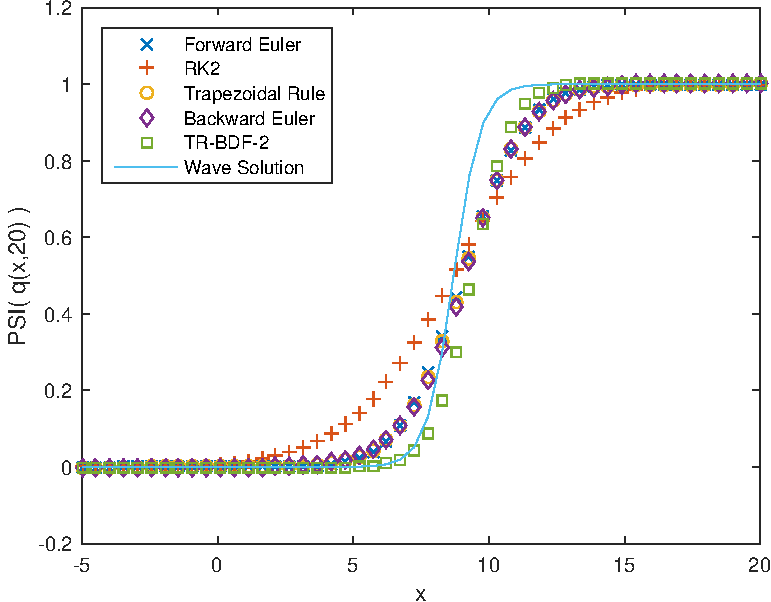
\includegraphics[width=0.5\textwidth]{figures/tau1e0.pdf}
            \caption{$\tau=10^{0}$}
        \end{figure}{}
        \vfill\null
        \columnbreak
        \begin{itemize}
            \item Everything is fine \\
        \end{itemize}{}
        \vfill\null
        \columnbreak
    \end{multicols}
\end{frame}{}




\begin{frame}{}
    \frametitle{Stability Issues}
    Results for different schemes after 20s simulation time
    \begin{multicols}{2}
         \begin{figure}
            \centering
            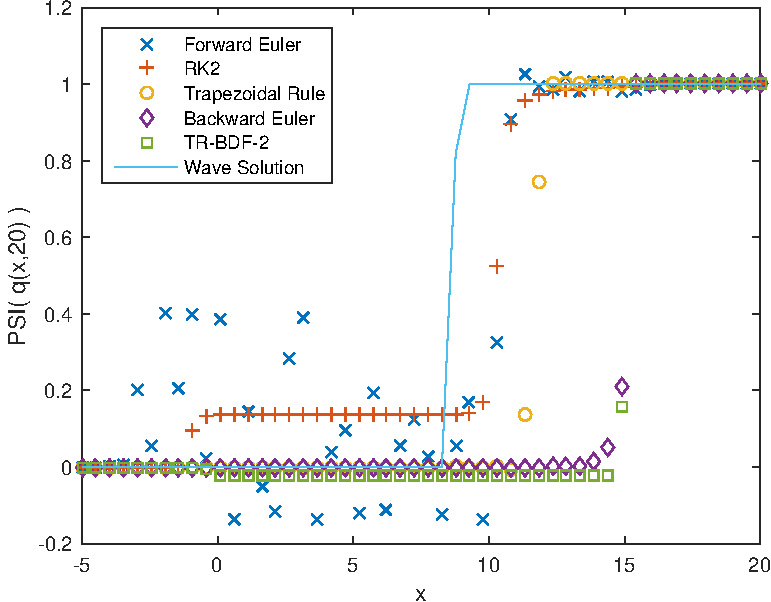
\includegraphics[width=0.5\textwidth]{figures/tau1e-1.pdf}
            \caption{$\tau=10^{-1}$}
        \end{figure}{}
         \vfill\null
        \columnbreak
       \begin{itemize}
            \item Explicit methods fail (except RK2) \\
            \item Implicit methods work fine \\
        \end{itemize}{}
        \vfill\null
        \columnbreak
    \end{multicols}
\end{frame}{}




\begin{frame}{}
    \frametitle{Stability Issues}
    Results for different schemes after 20s simulation time
    \begin{multicols}{2}
        \begin{figure}
            \centering
            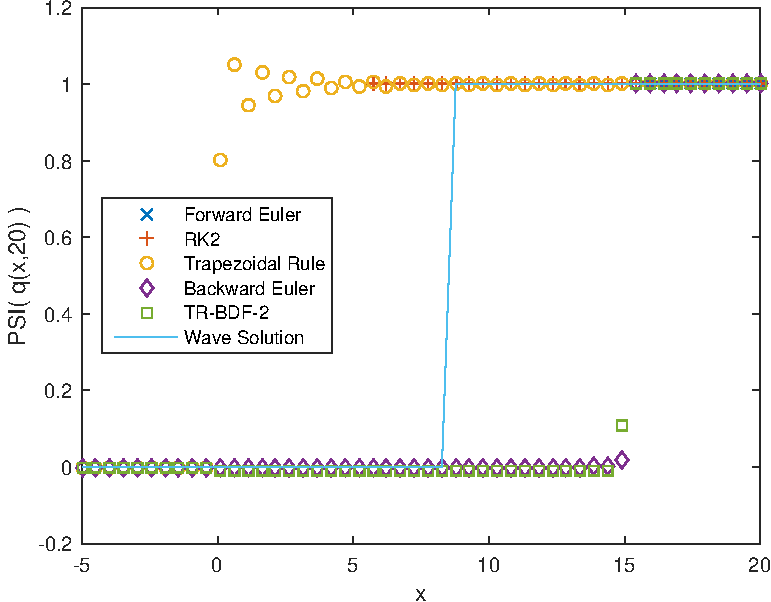
\includegraphics[width=0.5\textwidth]{figures/tau1e-2.pdf}
            \caption{$\tau=10^{-2}$}
        \end{figure}{}
        \vfill\null
        \columnbreak
        \begin{itemize}
            \item All explicit methods fail \\
            \item Trapezoidal rule fails (A-stable)\\
            \item Backwards Euler and TR-BDF2 work fine (L-stable)\\
        \end{itemize}{}
        \vfill\null
        \columnbreak
    \end{multicols}
\end{frame}{}






\begin{frame}{}
    \frametitle{Wrong Wave Propagation Speed}
    \vspace{1cm}
    \begin{multicols}{2}
        \begin{figure}
            \centering
            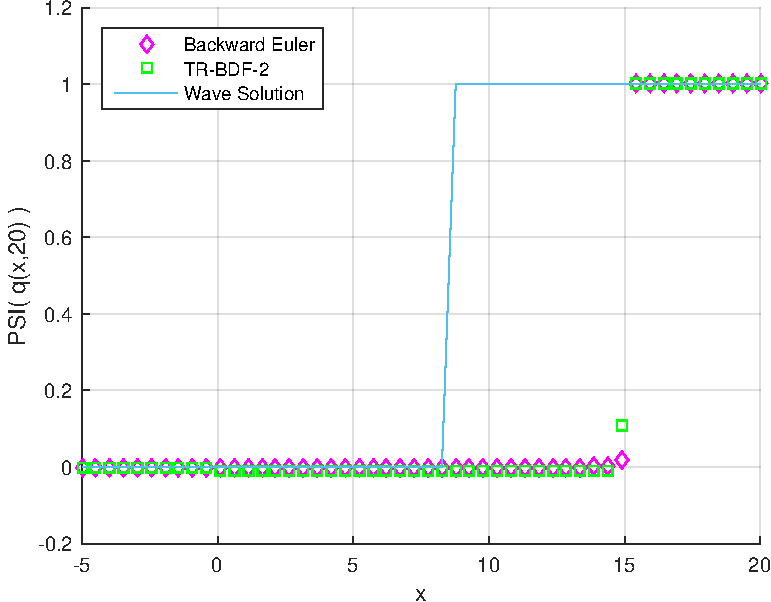
\includegraphics[width=0.5\textwidth]{figures/goombiwampi.pdf}
            \caption{Implicit solvers at $\tau=10^{-2}$}
            \label{fig:chupachups}
        \end{figure}{}
        \vfill\null
        \columnbreak  \pause
        We expect the wave travel speed to be $\beta=0.6$ \\
        We get a wave travel speed of $v=1$ \\
        This is due to the Godunov-Strang splitting: \\
        \begin{enumerate}
            \item Godunov scheme forces first non-zero value to a value below $\beta$
            \item The source term smears this value to 0
        \end{enumerate}
        The wave travels at 1 grid point per timestep \\
        As a result: unphysical wave propagation speed for stiff source terms
    \end{multicols}{}
\end{frame}{}

%%%%%%%%%%%%%%%%%%%%%%%%%%%%%%%%%%%%%%%%%%%%%%%%%%%%%%%%%%%%%%%%%%%%%%%%%%%%%%%%
\end{document} % !!! NICHT ENTFERNEN !!!
%%%%%%%%%%%%%%%%%%%%%%%%%%%%%%%%%%%%%%%%%%%%%%%%%%%%%%%%%%%%%%%%%%%%%%%%%%%%%%%%
